\documentclass[11pt,oneside,letterpaper]{article}

% graphicx package, useful for including eps and pdf graphics
\usepackage{graphicx}
\usepackage{grffile}
%\DeclareGraphicsExtensions{.pdf,.png,.jpg}

% basic packages
\usepackage{color}
\usepackage{parskip}
\usepackage{float}


% reference figures across documents
\usepackage{xr}
\externaldocument{mers-structure_supp}

% text layout
\usepackage{geometry}
\geometry{textwidth=15cm} % 15.25cm for single-space, 16.25cm for double-space
\geometry{textheight=22cm} % 22cm for single-space, 22.5cm for double-space

% helps to keep figures from being orphaned on a page by themselves
\renewcommand{\topfraction}{0.85}
\renewcommand{\textfraction}{0.1}

% bold the 'Figure #' in the caption and separate it with a period
% Captions will be left justified
\usepackage[labelfont=bf,labelsep=period,font=small]{caption}

% review layout with double-spacing
%\usepackage{setspace}
%\doublespacing
%\captionsetup{labelfont=bf,labelsep=period,font=doublespacing}

% cite package, to clean up citations in the main text. Do not remove.
%\usepackage{cite}
\usepackage{natbib}
%\renewcommand\citepleft{(}
%\renewcommand\citepright{)}
%\renewcommand\citepform[1]{\textsl{#1}}

\usepackage{amsmath}

% Remove brackets from numbering in list of References
%\renewcommand\refname{\large References}
%\makeatletter
%\renewcommand{\@biblabel}[1]{\quad#1.}
%\makeatother

\usepackage{authblk}
\renewcommand\Authands{ \& }
\renewcommand\Authfont{\normalsize \bf}
\renewcommand\Affilfont{\small \normalfont}
\makeatletter
\renewcommand\AB@affilsepx{, \protect\Affilfont}
\makeatother

% comments
\usepackage{ulem}
\definecolor{purple}{rgb}{0.459,0.109,0.538}
\def\tb#1#2{\sout{#1} \textcolor{purple}{#2}}
\def\tbc#1{\textcolor{purple}{[#1]}}

% symbols
\newcommand{\chiSq}{\chi^{2}_{df}}
\newcommand{\dtmrca}{\Delta_\mathrm{TMRCA}}
\newcommand{\undtmrca}{\delta_\mathrm{TMRCA}}
\newcommand{\dspr}{d_\mathrm{SPR}}

%%% TITLE %%%
\title{\vspace{1.0cm} \LARGE \bf Structured population models demystify MERS-CoV epidemiology}

\author[1]{Gytis Dudas}
\author[2]{Luiz Max Carvalho}
\author[1]{Allison Black}
\author[1]{Trevor Bedford}
\author[2,3,4]{Andrew Rambaut}

\affil[1]{Vaccine and Infectious Disease Division, Fred Hutchinson Cancer Research Center, Seattle, WA, USA}
\affil[2]{Institute of Evolutionary Biology, University of Edinburgh, Edinburgh, UK}
\affil[3]{Fogarty International Center, National Institutes of Health, Bethesda, MD, USA}
\affil[4]{Centre for Immunology, Infection and Evolution at the University of Edinburgh, Edinburgh, UK}

\date{\today}

\begin{document}
\maketitle

\begin{abstract}

Middle East Respiratory Syndrome coronavirus (MERS-CoV) is a zoonotic virus originating in camels that has been causing significant mortality and morbidity in humans in the Arabian Peninsula.
The epidemiology of the virus remains poorly understood, with hospital outbreaks, isolated cases with known exposure to camels and apparent community transmission occurring simultaneously.
Whilst traditional and seroepidemiological studies have been employed extensively throughout the epidemic, sequence data have not been utilised to any appreciable extent to understand transmission patterns within the entire outbreak.
Here we use existing MERS-CoV sequencing data to explore the phylodynamics of the virus in two of its major known hosts, humans and camels, as well as the interface between the two during cross species transmission.
We show that all of long-term MERS-CoV evolution occurs exclusively in camels, whereas humans act as the virus' terminal host.
Our study identifies MERS-CoV spillovers into humans as largely self-limiting, suggesting that curbing human exposure to camels or reducing the prevalence of the virus in camels are the most efficient ways of preempting future MERS outbreaks.
Joining a number of recent genomic epidemiology publications, our study highlights the utility of sequence data in understanding the transmission patterns of pathogens which are largely inaccessible to more traditional approaches.
\end{abstract}

\pagebreak

\section*{Introduction}
Middle East Respiratory Syndrome Coronavirus (MERS-CoV) is a zoonotic infection of humans in the Arabian Peninsula originating from camels.
The virus, first discovered in 2012 \citep{zaki_isolation_2012,boheemen_genomic_2012}, has gone on to cause more than 1800 infections with at least 600 associated deaths \citep{who_2016_MERS}.
Its epidemiology remains obscure, largely because outbreaks are observed among the most severely affected patients, such as older males with comorbidities \citep{assiri_2013,group_state_2013}.
Whilst contact with camels is often reported, many patients do not recall contact with any livestock, suggesting a significant but unobserved community contribution to the outbreak \citep{group_state_2013}.
Studies into MERS-CoV epidemiology in the past often relied on serology to identify factors associated with MERS-CoV exposure in potential risk groups \citep{reusken_occupational_2015,reusken_2013}.
Indeed, such data have been used to show high prevalence of past viral exposure in camels \citep{muller_2014,corman_antibodies_2014,chu_2014,reusken_2013,reusken_2014} and more frequent exposure in workers with occupational exposure to camels \citep{reusken_occupational_2015,muller_presence_2015} compared to the general population.
Traditional epidemiological approaches have also been used to look at distributions of case clusters through time, space and across hosts \citep{cauchemez_unraveling_2016}.


Although traditional approaches yield important clues about exposure patterns and potential for larger outbreaks, the origins of a pathogen remain opaque to traditional approaches.
The new era of genomic epidemiology, however, has repeatedly shown the utility of sequence data in outbreak scenarios \citep{arias_rapid_2016}.
Modern sequence data are relatively cheap to produce, can stand in for diagnostics and often yield a highly detailed picture of an epidemic when complete genome sequencing is performed consistently and appropriate metadata collected \citep{dudas_virus_2016}.
Often only sequence data can pinpoint sources of pathogens and discriminate between multiple and single source scenarios \citep{gire_genomic_2014}, which are fundamental to quantifying risk \citep{grubaugh_multiple_2017}.
Sequencing MERS-CoV has been performed as part of initial attempts to link human infections with the camel reservoir \citep{memish_human_2014}, nosocomial outbreak investigations \citep{assiri_hospital_2013} and routine surveillance \citep{park_acute_2015}.
A large portion of MERS-CoV sequences come from hospital outbreaks, where sequence data have been used to determine whether the introductions were of a single origin and homogenous or a result of increased cases among incoming patients \citep{fagbo_molecular_2015}.


It is widely accepted that recorded human MERS-CoV infections are a result of at least several introductions of the virus into humans \citep{cotten_2013}.
Previous studies attempting to quantify the actual number of spillover infections have either relied on traditional, and necessarily limited, approaches \citep{cauchemez_unraveling_2016} or relied on methods agnostic to underlying signals of population structure \citep{zhang_evolutionary_2016}.
Here we use existing MERS-CoV sequence data to investigate the population structure of the virus between two of its known hosts, humans and camels, as well as the zoonotic spillover dynamics at the interface between the two, by using an explicit model of population structure \citep{vaughan_efficient_2014}.
We show that viral evolution of MERS-CoV occurs almost exclusively in camels, where virus is also most likely to recombine.
Our results suggest that spillover events into humans appear to be considerably more common than previously thought.
Once human MERS-CoV infections are established, however, the virus has relatively poor person-to-person transmission and outbreaks are short-lived.
%\begin{figure}[h]
% \centering
%	\includegraphics[width=0.45\textwidth]{figures/}
%	\caption{\textbf{}
%
%	}
%	\label{}
%\end{figure}

\section*{Results}

\subsection*{MERS-CoV is predominantly a camel virus}
The structured coalescent approach we employ \citep{vaughan_efficient_2014} identifies the camel reservoir as the host population where most of MERS-CoV evolution takes place (see figure \ref{mcc}), whilst human MERS outbreaks are transient and terminal to the virus.
Across XXX MERS-CoV sequences collected from humans, we detect a median of XX individual camel to human cross-species transmissions (95\% highest posterior density: XX--XX).
Whilst we identify a median of X (95\% HPDs: X--XX) human-to-camel migrations, the 95\% HPD interval includes zero and we find that no such migrations are found in the maximum clade credibility tree (figure \ref{mcc}).
This suggests that these migrations are induced by the migration rate prior, rather than inferred from data.
The remainder of human-to-camel transmissions are likely derived from phylogenetic proximity of human sequences to the ``backbone'' of the phylogenetic tree.
It is most apparent in the lineages existing in early-mid 2013 that lead up to sequences comprising the MERS-CoV clade dominant in 2015, where poor sampling of MERS-CoV genetic diversity from camels allows the model to consider humans as a potential alternative host, given the proximity of sequences from humans to the ``backbone'' of the tree.
The first sequences of MERS-CoV from camels were collected in November 2013.

The repeated and asymmetric introductions of short-lived clusters of MERS-CoV sequences from camels into humans leads us to conclude that MERS-CoV epidemiology in humans is dominated by zoonotic transmission.
If MERS-CoV had attained any appreciable degree of community transmission we would expect to observe some continuity between human sequence clusters.
Yet we observe dense and terminal human clusters of MERS-CoV of no subsequent relevance to the evolution of the virus interspersed within the relatively large diversity of MERS-CoV lineages in camels.
In addition, these observations are derived from sequence data heavily skewed towards human cases and in all likelihood biased towards the most severe outbreaks documented.
We therefore argue that instances of human infection with MERS-CoV are more common than currently thought, with exceedingly short transmission chains mostly limited to index cases, and probably, on average, milder pathology that do not get reported, let alone sequenced.

% We also detect apparent seasonality in times of zoonotic transfer of viruses.
% Whilst zoonotic transmissions occur throughout the entire year, particularly large sequence clusters begin as viral introductions into humans earlier in the year.
% %We identify
% There is also apparent heterogeneity in resulting human cluster sizes, which is not unexpected.
% Large clusters of MERS are apparent and mostly correspond to known large transmission chains, often in a nosocomial setting, such as the outbreak in South Korea and Riyadh.
% At the same time, the long tail of the sequence cluster size distribution is an indicator of transmission chains terminating soon after introduction, many of which could represent genuine singleton infections.

\subsection{MERS-CoV is poorly suited for human transmission}
Whilst the structured coalescent model clearly shows humans as a terminal host for MERS-CoV, we want to quantify this further.

This explains why MERS-CoV has not caused a detectable general epidemic in the Arabian Peninsula, nor a world-wide pandemic.

%\begin{figure}[h]
% \centering
%	\includegraphics[width=0.65\textwidth]{figures/}
%	\caption{\textbf{}
%
%	}
%	\label{}
%\end{figure}

\begin{figure}[h]
 \centering
	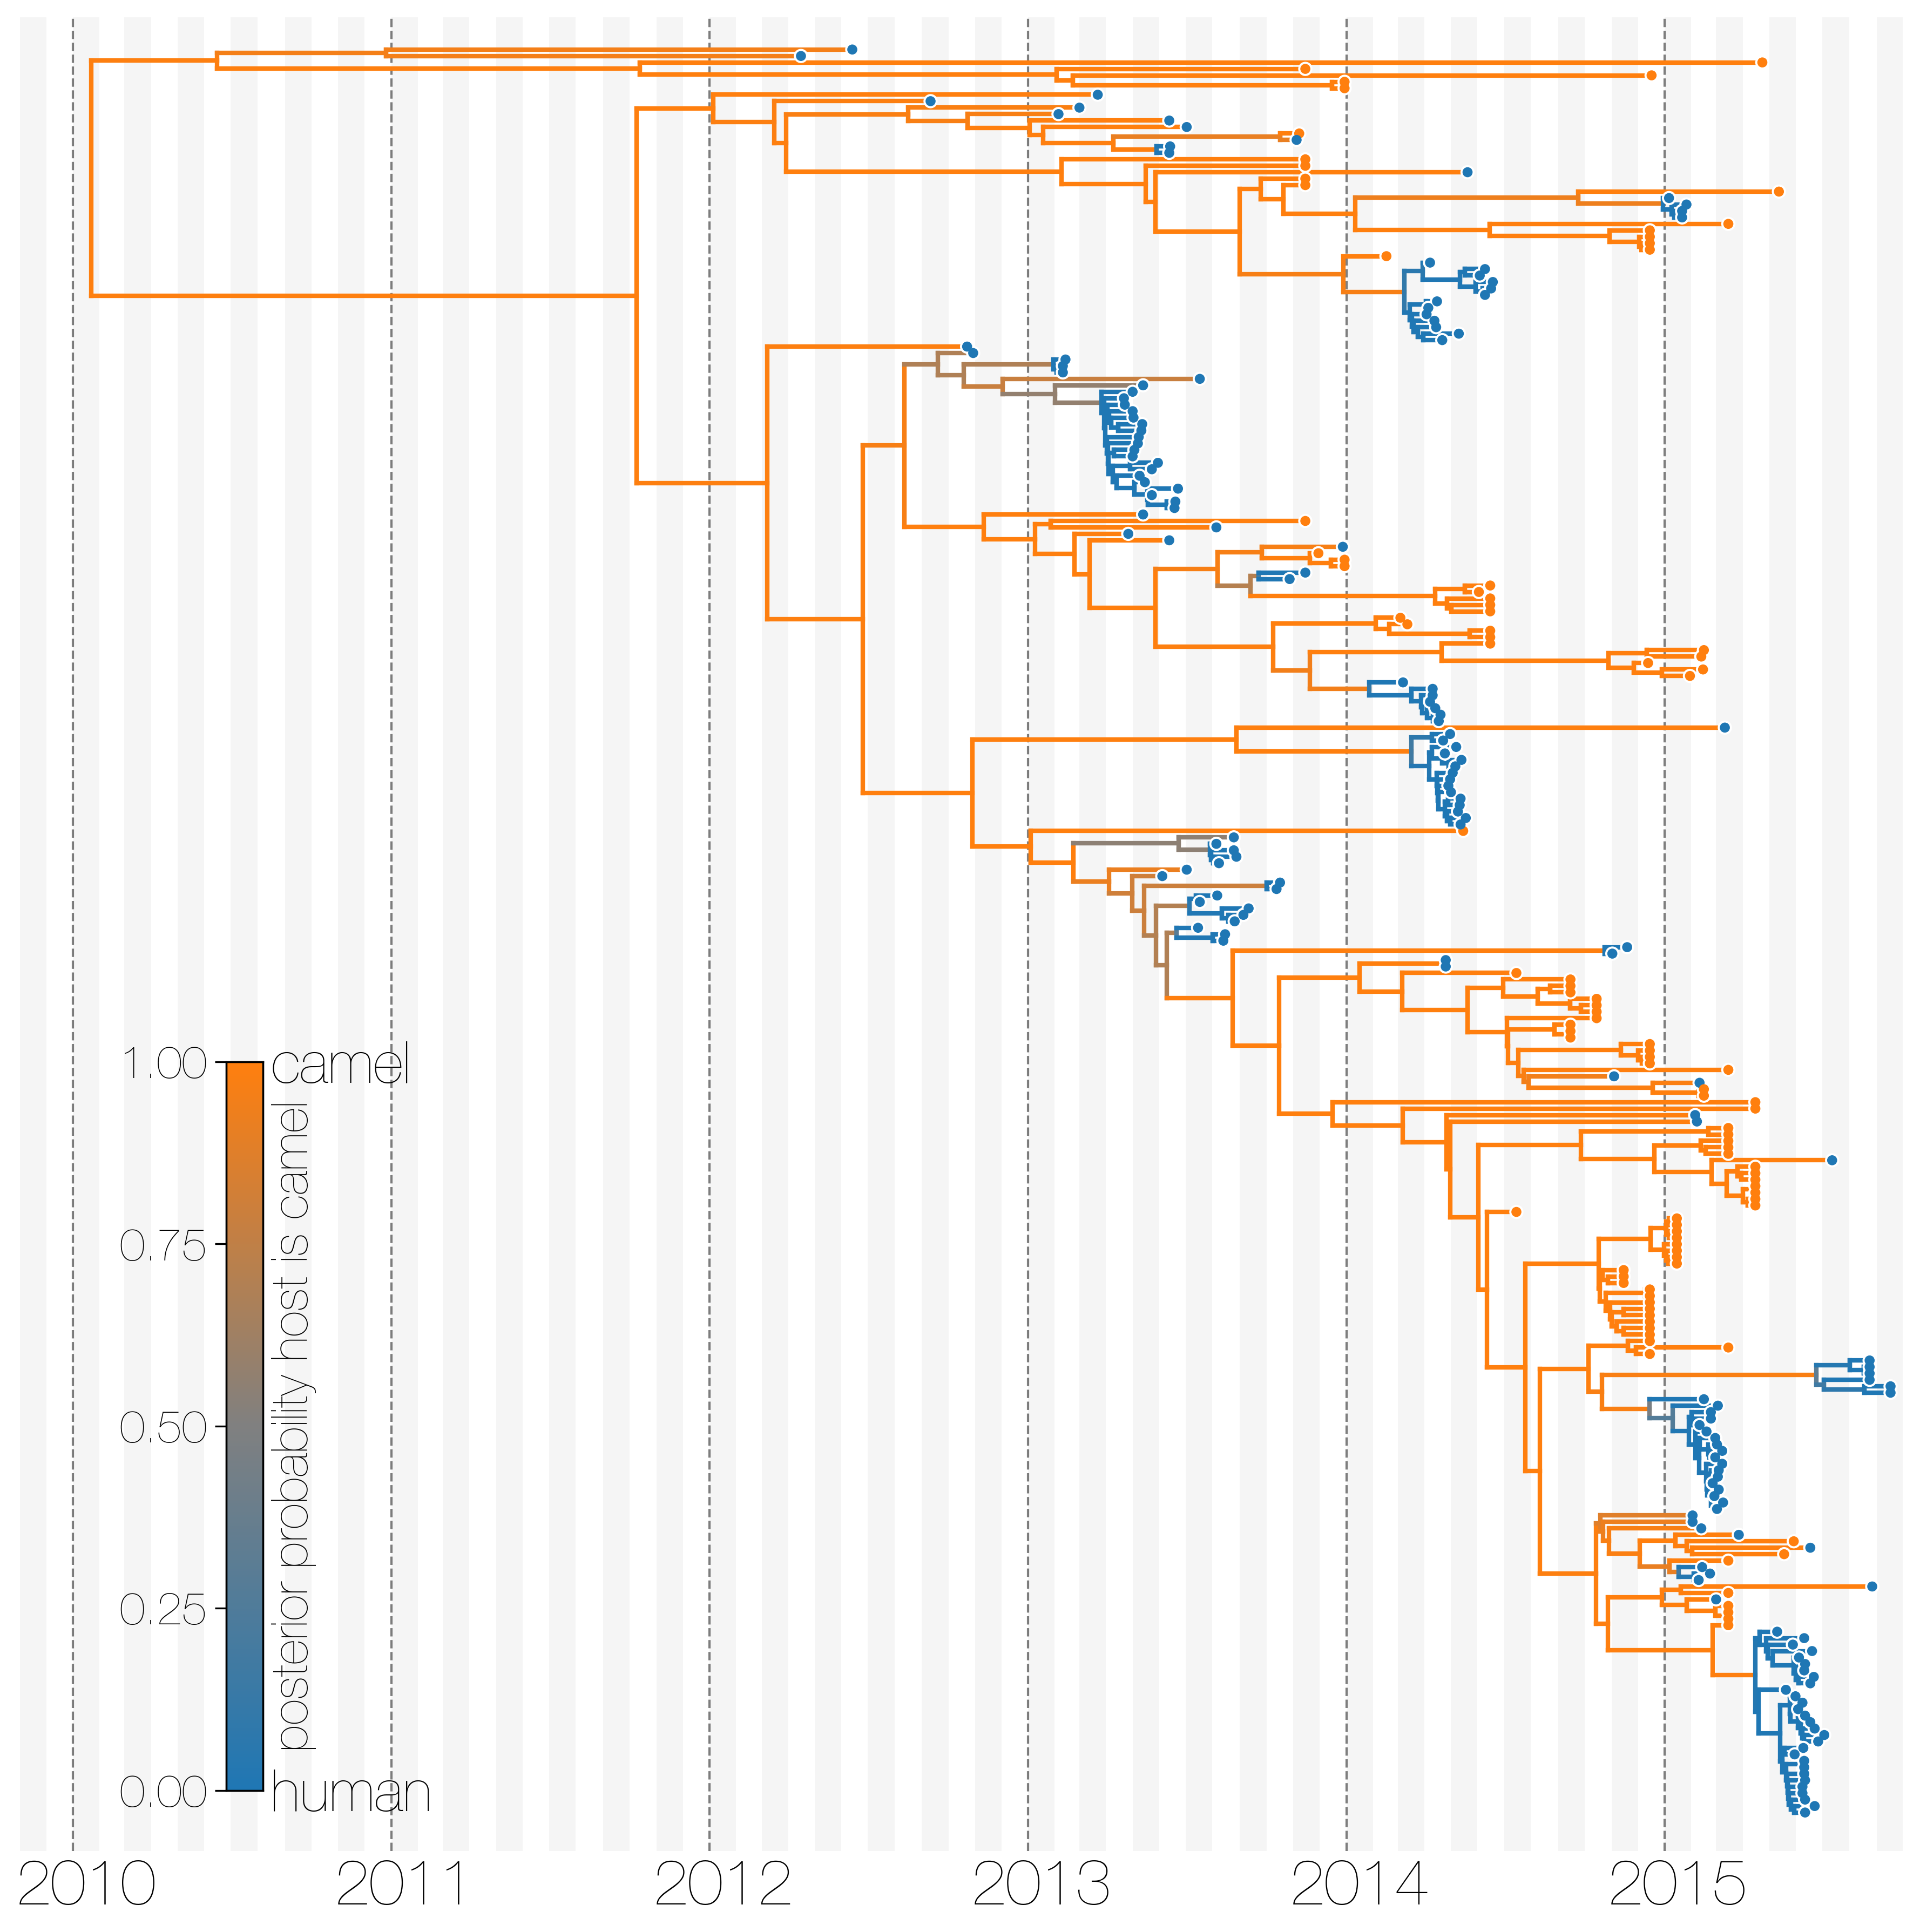
\includegraphics[width=0.65\textwidth]{figures/mers_mcc.png}
	\caption{\textbf{Typed maximum clade credibility tree of MERS-CoV sequences from humans and camels.}
	Maximum clade credibility (MCC) tree showing inferred ancestral hosts for MERS-CoV recovered using the structured coalescent.
	Vast majority of MERS-CoV evolution is inferred to occur in camels (orange) with human outbreaks (blue) representing evolutionary dead-ends for the virus.
  Confidence in host assignment is depicted as a colour gradient, with increased uncertainty in host assignment (posterior probabilities close to 0.5) shown as grey.
	Whilst large clusters of human cases are apparent in the tree, significant contributions to human outbreaks are made by singleton sequences, likely representing recent cross-species transmissions that were caught early.
	}
	\label{mcc}
\end{figure}



\subsection*{Recombination shapes MERS-CoV diversity}
Recombination has been shown to occur in all genera of coronaviruses, including MERS-CoV.
In order to explore the role of recombination in shaping MERS-CoV genetic diversity we used two recombination detection approaches across partitions of data corresponding to inferred MERS-CoV clades.
Both methods used rely on sampling parental and recombinant alleles within the alignment, although each quantifies different signals of recombination.
One hallmark of recombination is the ability to carry alleles derived via mutation from one lineage to another, which gives the appearance of repeated mutations taking place in the recipient lineage, somewhere else in the tree.
PHI (pairwise homoplasy index) test quantifies the appearance of these excessive repeat mutations (homoplasies) within an alignment.
Another hallmark of recombination is spatial clustering of alleles in the genome, due to how template switching, the primary mechanism of recombination in RNA viruses, occurs.
3Seq relies on the spatial structure of nucleotide similarities between sequence triplets -- two potential parent-donors and one candidate offspring-recipient sequences.

Both tests can give spurious results in cases of extreme rate heterogeneity \citep{dudas_mers-cov_2016}, but both are not known to fail simultaneously.
PHI and 3Seq methods consistently identify most of the apparent `backbone' of the phylogeny as encompassing sequences with evidence of recombination (figure \ref{mcc}).
Neither method can identify where in the tree recombination occurred, but each full asterisk in figure \ref{mcc} should be interpreted as the minimum partition of data that still captures recombinant descendants.
This suggests a non-negligible contribution of recombination in shaping existing MERS-CoV diversity.

Amongst clusters inferred to be infecting humans we see extremely limited amounts of genetic diversity, accompanied by fewer homoplasies (figure \ref{}).
Given that recombination requires co-infection with two or more distinct lineages of the virus, the low prevalence of the MERS-CoV in the general human population, and its poor transmissibility, there is little reason to suspect that distinct MERS-CoV lineages are able to generate widespread recombination we observe.
This is reassuring, since phylogenetic approaches can be used freely in these scenarios, but limiting analysis to sequences strictly from single-introduction clusters comes at a cost of mutational resolution.
In contrast, the prevalence of MERS-CoV in camels is thought to be high, camels seemingly suffer only mild symptoms from infection and most of MERS-CoV evolutionary history takes place in camels.
This makes camels the ideal host where distinct lineages of MERS-CoV can frequently mingle and recombine as a consequence.


% Here we confirm this assumption by showing that evolution of MERS-CoV within human clusters is clonal.
% This is not surprising, since zoonotic transmission of MERS-CoV into humans is relatively rare, of limited diversity at the point of introduction and viral diversity in humans is ultimately transient.
% All of these factors act to make co-infection of humans with MERS-CoV exceedingly rare.
% It is worth highlighting that MERS-CoV almost certainly recombines during human infection, but the limited diversity of virus populations in individual humans renders it invisible and of little consequence.
%
% Although we do not detect recombination in human clusters, we see evidence for introduction of recombinant viruses into humans which evolve clonally after the transfer (figure \ref{chain}).
% This is not unexpected either - there are strong indications that the Korean MERS outbreak was caused by a recombinant virus crossing the species barrier.
% The frequency of MERS-CoV recombination in the reservoir implies that co-infection of camels is quite common, and by extension that the virus is likely to be very prevalent in this host.

\begin{figure}[h]
 \centering
	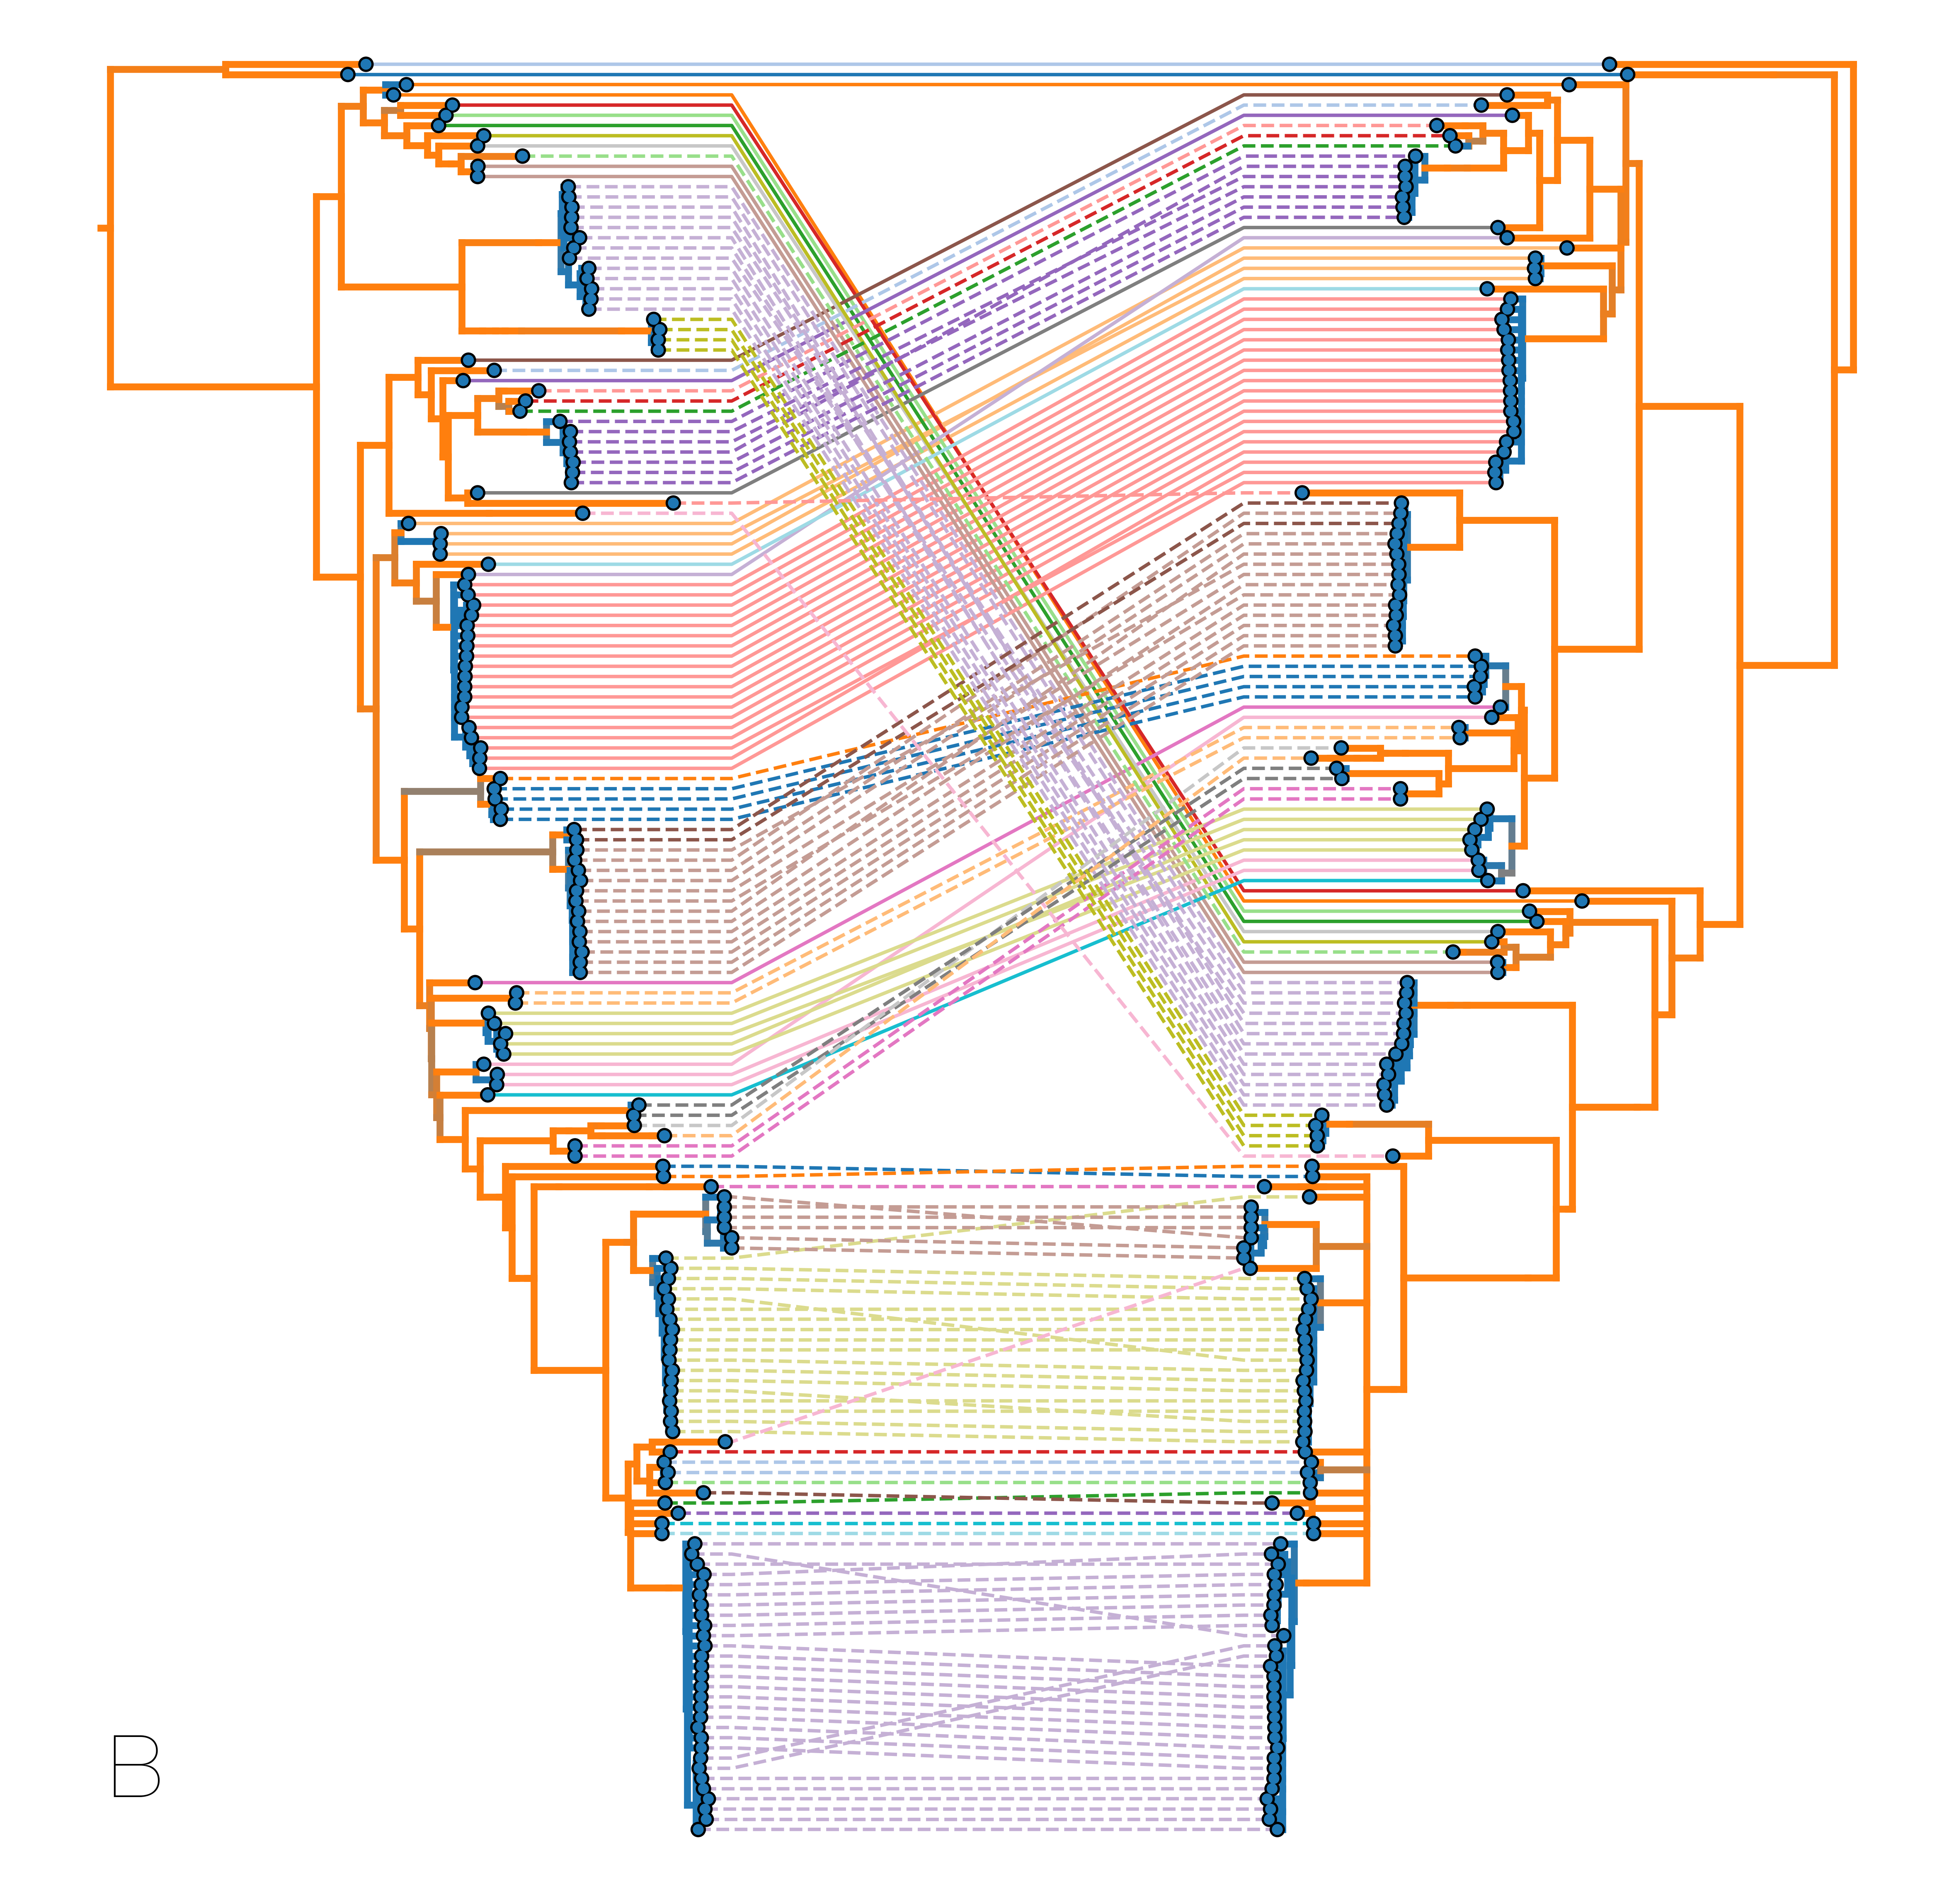
\includegraphics[width=0.65\textwidth]{figures/mers_chain.png}
	\caption{\textbf{Tangled chain of MERS-CoV genome and its parts.}
	Tangled chain of the full genome (a), all nucleotides up to position 21000 (b) and all nucleotides past position 21000 (c) of MERS-CoV.
	The same taxa, if available in neighbouring trees, are connected via coloured lines (human sequences in blue, camel sequences in red).
	Tree branches are coloured by inferred ancestral host state (human in grey, camel in black).
	Whilst some of apparent incongruities are caused by having less data in some of the fragments, inconsistencies between topologies occur across internal branches inferred to be in the camel host.
	Human clusters in grey change phylogenetic positions between the trees wholesale, with minor incongruences within clusters.
	This is evidence for recombinant viruses generated in the reservoir entering human populations.
	Coding sequences in the MERS-CoV genome are indicated with arrows at the bottom of the plot with position 21000 indicated by the black line.
	}
	\label{fig:mers_chain}
\end{figure}

% \subsection*{Effects of recombination are minimal on human clusters}
% Most phylogenetic approaches model sequence evolution as a strictly clonal process and when recombination is present traditional phylogenetic approaches can fail to recover correct topologies, branch lengths or demographic history.
% All coronavirus genera are known to be recombinogenic and MERS-CoV is no exception.
% Whereas recombination is obligate for some eukaryotes, detectable RNA virus recombination can only occur during co-infection with two or more distinct viral genotypes.
% Previous studies have inferred prevalent recombination in MERS-CoV \citep{dudas_mers-cov_2016} and found direct evidence for it \citep{}.
% When not directly looking for recombination, however, most studies carried out their objectives without regard for potential effects of recombination.
% Our independent analyses of the alignment split into two fragments reveals that effects of recombination are certainly detectable, but limited to the parts of the phylogeny evolving in camels.
%So whereas we find some evidence of recombinant viruses crossing the species barrier into humans


% \subsection*{MERS epidemiology}





% Although sequences in an outbreak necessarily represent a subset of all the cases, their clustering and resulting cluster sizes can be highly informative of underlying epidemiological processes that are otherwise inaccesible or unfeasible to study.
% In our case we have used sequence data to disentangle the evolution of MERS-CoV into two discrete host compartments.
% By removing the confounding effects of shared ancestry for MERS-CoV sequences we can treat every viral introduction into humans as an independent replicate of the transmission process in humans.


\section*{Discussion}

\subsection{Population structure and inference}
Phylogeny labelling approaches depend on discrete states being assigned to taxa, followed by ancestral state reconstruction equivalent to that applied to nucleotide sites.
These methods, when used to infer ancestral migration history across a phylogeny, have thus been called ``mugration'' models.
When the number of possible discrete states is limited, data are ample and questions are formulated correctly, phylogeny labelling approaches are computationally efficient.
However, ``mugration'' models ignore potentially relevant information, such as markedly different demographic histories under across distinct populations.

Sequencing of MERS-CoV has been a challenging issue, especially from the reservoir.
MERS-CoV seroprevalence in camels, as expected of a reservoir, is very high, yet sequencing efforts have overwhelmingly focused on human infections.
At present MERS-CoV sequences collected from humans outnumber those from camels at a ratio of over 2-to-1, and camel sequences make a late appearance in our data, largely because of the time required to identify camels as the reservoir for the virus.
Using such data in a ``mugration'' model have led to proposals that MERS-CoV is an epizootic in camels of largely human origins \citep{zhang_evolutionary_2016}, a finding that contradicts other sources of information.
Similarly, traditional epidemiological approaches have no way of firmly establishing links between human cases outside of known family clusters or hospital outbreaks \citep{cauchemez_unraveling_2016}.

Our study has shown how significantly different demographic regimes can be leveraged against biased sequence data to arrive at conclusions perfectly in line with prior observations.
It has been apparent for some time that MERS-CoV sequences collected from camels are, on average, relatively distantly related to each other, whereas human outbreaks tended to fall into densely sampled clusters of no apparent relation or consequence to further human outbreaks.
These hallmarks of distinct demographic modes were easily picked up by the explicit population structure model we employed, and helped us arrive at a comprehensive picture of MERS-CoV epidemiology in agreement with previous empirical studies.


\subsection*{MERS-CoV epidemiology}
Our analyses firmly support camels as the primary and essential host of human MERS coronaviruses.
Although sequencing efforts for MERS-CoV have been highly human-biased, we have found that over 80\% of the sampled MERS-CoV evolutionary history has occurred in camels.
In contrast, sequences recovered from human cases represent MERS-CoV lineages that play no detectable role in the long-term evolution of the virus.
The difference in apparent host suitability between humans and camels helps explain why unlike some human viruses of zoonotic origins, such as Ebola virus, that have spread internationally, MERS-CoV has remained a problem largely limited to the Arabian Peninsula.
The sole exception to this has been the MERS outbreak in South Korea.


%Despite the crucial role camels play in MERS-CoV maintenance, we have also identified a relatively small effective population size of the virus in the camel reservoir.


% Our observation of recombinant MERS coronaviruses being transmitted to humans is not cause for concern by itself, however, the mere presence of detectable recombination implies that co-infection of camels with MERS-CoV is common.
% By extension, frequent co-infection implies a high prevalence of the virus in camels, which is the main unsettling conclusion.
% There is ample evidence for this from seroepidemiology, which has shown that XX\% of camels are infected by age XX.
% Our results show that zoonotic transmission of MERS-CoV into humans is the main drivers for the continuation of the outbreak in the Arabian Peninsula.
% Prevalence of MERS-CoV in camels could easily be translated into force of infection and given the role of zoonotic transmission as the main driver for the outbreak only reiterates the importance of controlling the MERS coronavirus in the reservoir if the human side of the outbreak is to be brought under control.


\subsection*{Issues with recombination}
Recombination in MERS-CoV is now an accepted feature of the system.
Prevalent recombination can seriously impede phylogenetic and other sequence analysis techniques.
We argue that although MERS-CoV sequences contain overwhelming evidence for recombination, we do not expect humans to play a major role in this process.
Every introduction of the virus into a human population is expected to establish an apparently clonally evolving population.
However, lineages crossing the species barrier are very likely to have experienced recombination at some point in their past, in some cases occurring right before zoonotic transmission, as was the case in the Korean outbreak of MERS.
We thus conclude that whilst sequence analyses of MERS-CoV are perfectly legitimate for well-defined human outbreaks, extreme care must be taken when inferring their origins in the context of the reservoir, or even when comparing related outbreaks in humans.
We also strongly advise against drawing hasty conclusions from MERS-CoV phylogenies recovered from human sequences if they span more than four months of evolution or camel sequences under virtually all circumstances, as there is no guarantee that phylogenies will cover the clonal evolutionary history of the virus in humans.


\newpage

\section*{Methods}
\subsection*{Sequence data}
All MERS-CoV sequences were downloaded from GenBank.
Fragments of some strains submitted to GenBank as separate accessions were assembled into a single sequence.
Protein coding sequences were extracted and concatenated.
Sequences were annotated with available collection dates and hosts, designated as camel or human.
For partitioned analyses the alignment was split into two fragments, the first containing all nucleotides up to nucleotide 21000, and the rest of the genome being assigned to the second fragment.
Despite their divergence both Severe Acute Respiratory Syndrome (SARS) and MERS betacoronaviruses appear to recombine across position 21000, which may indicate the existence of a recombinogenic secondary RNA structure that remains to be described in its vicinity. %% "Work by Zhang et al. (66) suggested that the presence of a stable hairpin between two direct repeats increases the rate of homologous recombination in MLV. Their data led to the conclusion that stable secondary structures decrease processive RT synthesis and, further, that a functional NC can increase RT processivity. However, in this case, there were no corresponding in vitro data (such as primer extension assays) to correlate with the in vivo observations. Here, we have demonstrated for the first time a direct relationship between pausing in vitro and viral recombination in vivo."

\subsection*{Structured coalescent analyses}
MultiTypeTree module \citep{vaughan_efficient_2014} was used in BEAUti v2.4.3 \citep{bouckaert_beast_2014} to specify a structured coalescent model with two demes - humans and camels - based on GenBank records.
Analyses were run on codon position partitioned data with two separate HKY+$\Gamma_{4}$ \citep{hky_1985,yang_1994} nucleotide substitution models specified for codon positions 1+2 and 3.
A relaxed molecular clock with branch rates drawn from a lognormal distribution \citep{drummond_2006} was used to infer the evolutionary rate from date calibrated tips.
Default priors were used for all parameters except for migration rates between demes for which an exponential prior with mean 1.0 was used.
An identical set up was used for analysing alignments split into two fragments, with independent clocks, trees and migration rates, but shared substitution models and deme population sizes.
Eight independent whole-genome MCMC analyses were run, for 200 million states each subsampling every 20000 states.
For two-fragment MCMC analyses ten independent runs were set up.
Due to the increased complexity of multitype tree parameter space 50\% of states from every analysis were discarded as burnin.

\subsection*{Epidemiological analyses}


\begin{equation}
p(r = j | R_{0}, \omega) = \frac{\Gamma(\omega j+j-1)}{\Gamma(\omega j)\Gamma(j+1)} \frac{(\frac{R_{0}}{\omega})^{j-1}}{(1+\frac{R_{0}}{\omega})^{\omega j+j-1}}
\end{equation}

\subsubsection*{Introduction seasonality}
We computed the times of camel-to-human introductions in the posterior distribution of trees.
This distribution of introduction times was then discretised as follows: for state  $k = 1, 2, \ldots, L$ in the chain,  $Z_{ijk}$ was $1$ if there as an introduction in month $i$ and year $j$ and $0$ otherwise.
We model the variable $Y_{ij} = \sum_{k = 1}^M Z_{ijk}$ with the hierarchical model:
\begin{align}
 Y_{ij} &\sim \text{Binomial}(L, \theta_{ij}); \\
 logit(\theta_{ij}) &= \alpha_j + \beta_i; \\
 \beta_i &\sim \text{Normal}(0, \sigma_{m}); \\ 
  \sigma_{m} &\sim \text{Cauchy}(0, 2.5); \\
 \alpha_j &\sim \text{Normal}(\mu_{y}, \sigma_{y});  \\
 \mu_{y}  &\sim  \text{Normal}(0, 1); \\
 \sigma_{y} &\sim \text{Cauchy}(0, 2.5).
\end{align}


\subsection*{Data availability}


\section*{Acknowledgements}

\bibliographystyle{mbe.bst}
\bibliography{mers-structure}

\end{document}
